\chapter*{Apendix}
\addcontentsline{toc}{chapter}{Apendix}

\section*{Apendix A}
Následující tabulka zachycuje informace o vyhodnoceních diskretizačního
algoritmu nad jednotlivými tunely. V prvním sloupci nalezneme kódové označení
proteinu, ve kterém se daný tunel nachází. Druhý sloupec říká kolika koulemi byl
tunel aproximován a třetí sloupec kolik řezů algoritmus vygeneroval. Čtvrtý
resp. pátý sloupec značí dobu trvání preprocessing fáze resp. celkový čas výpočtu
v sekundách.
\begin{table}[htbp]
    \centering
    \fontsize{9}{11}\selectfont
    \begin{tabular}{||c | c c c c||}
        \hline
        Code & SC & DC & PT & TT \\ [0.5ex]
        \hline\hline
        1A9X & 12 & 49 & 5.8 & 8.1 \\
        \hline
        1A9X & 23 & 106 & 13.9 & 19.9 \\
        \hline
        1A9X & 27 & 131 & 17.2 & 23.4 \\
        \hline
        1AKD & 15 & 68 & 5.0 & 7.6 \\
        \hline
        1AKD & 16 & 71 & 5.8 & 8.7 \\
        \hline
        1AKD & 18 & 80 & 8.5 & 11.7 \\
        \hline
        1B37 & 10 & 45 & 3.5 & 5.3 \\
        \hline
        1B37 & 21 & 98 & 11.9 & 16.4 \\
        \hline
        1B37 & 26 & 132 & 14.9 & 20.1 \\
        \hline
        1B37 & 28 & 130 & 14.7 & 21.1 \\
        \hline
        1B37 & 29 & 132 & 17.0 & 23.4 \\
        \hline
        1B37 & 29 & 145 & 19.2 & 26.0 \\
        \hline
        1B37 & 29 & 146 & 16.9 & 22.4 \\
        \hline
        1B37 & 35 & 170 & 21.7 & 28.9 \\
        \hline
        1B37 & 36 & 169 & 22.1 & 31.3 \\
        \hline
        1B37 & 40 & 202 & 35.5 & 46.9 \\
        \hline
        1B37 & 46 & 220 & 35.8 & 46.8 \\
        \hline
        1BL8 & 43 & 183 & 40.1 & 54.6 \\
        \hline
        1BN7 & 14 & 57 & 5.8 & 8.9 \\
        \hline
        1BN7 & 19 & 83 & 8.8 & 12.4 \\
        \hline
        1BRT & 25 & 133 & 12.7 & 17.1 \\
        \hline
        1BRT & 46 & 216 & 33.4 & 44.8 \\
        \hline
        1BRT & 52 & 234 & 40.9 & 54.9 \\
        \hline
        1EA5 & 22 & 114 & 14.0 & 18.4 \\
        \hline
        1EA5 & 34 & 174 & 26.2 & 33.4 \\
        \hline
        1H2W & 20 & 103 & 11.7 & 16.2 \\
        \hline
        1H2W & 31 & 174 & 31.5 & 39.9 \\
        \hline
        1H2W & 35 & 183 & 30.3 & 40.4 \\
        \hline
        1H2W & 35 & 218 & 39.8 & 49.2 \\
        \hline
        1H2W & 38 & 223 & 45.3 & 55.1 \\
        \hline
        1H2W & 39 & 211 & 44.3 & 55.5 \\
        \hline
        1H2W & 39 & 243 & 45.0 & 61.5 \\
        \hline
    \end{tabular}
    \hfill
    \begin{tabular}{||c | c c c c||}
        \hline
        Code & SC & DC & PT & TT \\ [0.5ex]
        \hline\hline
        1H2W & 40 & 210 & 34.9 & 44.9 \\
        \hline
        1H2W & 41 & 238 & 49.1 & 61.4 \\
        \hline
        1H2W & 41 & 240 & 49.7 & 65.5 \\
        \hline
        1H2W & 44 & 246 & 56.5 & 71.2 \\
        \hline
        1H2W & 46 & 287 & 55.4 & 70.7 \\
        \hline
        1H2W & 50 & 294 & 64.3 & 85.8 \\
        \hline
        1HFE & 20 & 100 & 13.0 & 16.3 \\
        \hline
        1HFE & 21 & 90 & 10.0 & 14.3 \\
        \hline
        1HFE & 28 & 132 & 16.2 & 22.1 \\
        \hline
        1HFE & 38 & 193 & 24.4 & 33.0 \\
        \hline
        1HFE & 45 & 223 & 35.5 & 47.4 \\
        \hline
        1HNJ & 12 & 60 & 3.7 & 6.3 \\
        \hline
        1HNJ & 24 & 109 & 12.7 & 18.4 \\
        \hline
        1HNJ & 42 & 208 & 31.6 & 42.0 \\
        \hline
        1I88 & 12 & 52 & 4.5 & 6.7 \\
        \hline
        1I88 & 25 & 120 & 15.8 & 20.9 \\
        \hline
        1I88 & 27 & 139 & 18.1 & 23.4 \\
        \hline
        1I88 & 27 & 140 & 16.2 & 22.8 \\
        \hline
        1I88 & 36 & 187 & 27.6 & 35.8 \\
        \hline
        1M1N & 14 & 72 & 4.9 & 7.3 \\
        \hline
        1M1N & 32 & 155 & 19.1 & 27.0 \\
        \hline
        1M1N & 33 & 155 & 21.3 & 28.3 \\
        \hline
        1MHY & 21 & 100 & 9.9 & 14.3 \\
        \hline
        1MHY & 46 & 218 & 42.0 & 54.3 \\
        \hline
        1MHY & 59 & 304 & 57.6 & 73.1 \\
        \hline
        1MHY & 60 & 291 & 65.0 & 83.0 \\
        \hline
        1MHY & 60 & 306 & 61.0 & 80.1 \\
        \hline
        1MHY & 69 & 340 & 78.9 & 104.0 \\
        \hline
        1MHY & 70 & 348 & 83.1 & 105.0 \\
        \hline
        1MKB & 19 & 91 & 9.6 & 14.3 \\
        \hline
        1MKB & 30 & 148 & 19.8 & 25.7 \\
        \hline
        1MQF & 12 & 53 & 4.2 & 6.3 \\
        \hline
    \end{tabular}
    \caption{Tabulka evaluace diskretizačního algoritmu.}
\end{table}
\begin{table}
    \fontsize{9}{11}\selectfont
    \begin{tabular}{||c |c c c c||}
        \hline
        Code & SC & DC & PT & TT \\ [0.5ex]
        \hline\hline
        1MQF & 17 & 78 & 9.2 & 13.9 \\
        \hline
        1MQF & 24 & 117 & 18.5 & 23.8 \\
        \hline
        1MXT & 19 & 89 & 11.9 & 16.7 \\
        \hline
        1MXT & 19 & 98 & 11.1 & 14.9 \\
        \hline
        1MXT & 33 & 164 & 28.0 & 37.1 \\
        \hline
        1PBE & 16 & 70 & 6.5 & 9.7 \\
        \hline
        1PBE & 18 & 89 & 6.9 & 10.7 \\
        \hline
        1PBE & 19 & 81 & 8.5 & 12.3 \\
        \hline
        1PBE & 28 & 146 & 17.6 & 23.0 \\
        \hline
        1PBE & 34 & 170 & 23.1 & 30.2 \\
        \hline
        1SU8 & 18 & 93 & 7.9 & 11.4 \\
        \hline
        1SU8 & 30 & 143 & 19.3 & 26.2 \\
        \hline
        1SU8 & 35 & 172 & 27.0 & 34.7 \\
        \hline
        1SU8 & 39 & 185 & 28.0 & 37.7 \\
        \hline
        1SU8 & 47 & 236 & 45.1 & 57.4 \\
        \hline
        1SU8 & 47 & 242 & 43.4 & 55.3 \\
        \hline
        1SU8 & 9 & 38 & 2.2 & 3.8 \\
        \hline
        1THG & 11 & 45 & 3.7 & 5.5 \\
        \hline
        1THG & 12 & 51 & 5.1 & 7.3 \\
        \hline
        1THG & 14 & 68 & 5.5 & 8.3 \\
        \hline
        1VA4 & 11 & 49 & 3.5 & 5.2 \\
        \hline
        1VA4 & 15 & 71 & 5.6 & 7.7 \\
        \hline
        1VA4 & 18 & 75 & 9.0 & 12.6 \\
        \hline
        1YGE & 120 & 588 & 196.0 & 261.4 \\
        \hline
        1YGE & 30 & 146 & 21.7 & 27.9 \\
        \hline
        1YGE & 30 & 155 & 18.3 & 24.2 \\
        \hline
        1YGE & 33 & 160 & 19.7 & 26.8 \\
        \hline
        1YGE & 45 & 240 & 38.1 & 48.7 \\
        \hline
        1YGE & 51 & 264 & 43.5 & 56.0 \\
        \hline
        1YGE & 53 & 247 & 42.9 & 58.4 \\
        \hline
        1YGE & 90 & 445 & 109.8 & 149.6 \\
        \hline
        1YQW & 30 & 147 & 17.9 & 23.9 \\
        \hline
        1YRC & 14 & 64 & 6.0 & 9.3 \\
        \hline
        1YRC & 25 & 136 & 15.2 & 20.8 \\
        \hline
        1YRC & 28 & 138 & 21.0 & 28.7 \\
        \hline
        2ACE & 11 & 52 & 3.5 & 6.4 \\
        \hline
        2ACE & 13 & 65 & 7.7 & 11.2 \\
        \hline
        2ACE & 18 & 78 & 8.6 & 12.4 \\
        \hline
        2AYL & 25 & 122 & 14.6 & 20.3 \\
        \hline
        2AYL & 34 & 170 & 21.7 & 28.7 \\
        \hline
        2AYL & 35 & 176 & 20.9 & 27.3 \\
        \hline
        2AYL & 36 & 172 & 24.3 & 32.0 \\
        \hline
        2AYL & 39 & 193 & 28.6 & 38.2 \\
        \hline
        2AYL & 41 & 201 & 30.5 & 41.4 \\
        \hline
    \end{tabular}
    \hfill
    \begin{tabular}{||c | c c c c||}
        \hline
        Code & SC & DC & PT & TT \\ [0.5ex]
        \hline\hline
        2AYL & 47 & 225 & 37.3 & 50.8 \\
        \hline
        2AYL & 49 & 249 & 47.1 & 60.8 \\
        \hline
        2AYL & 54 & 280 & 46.5 & 61.4 \\
        \hline
        2BG9 & 139 & 833 & 529.2 & 667.2 \\
        \hline
        2C3N & 15 & 70 & 5.0 & 8.4 \\
        \hline
        2C3N & 20 & 89 & 9.8 & 13.2 \\
        \hline
        2C3N & 25 & 113 & 11.6 & 15.7 \\
        \hline
        2IID & 19 & 97 & 9.4 & 12.7 \\
        \hline
        2IID & 20 & 102 & 10.4 & 14.6 \\
        \hline
        2IID & 20 & 93 & 11.4 & 16.1 \\
        \hline
        2IID & 21 & 100 & 11.3 & 15.3 \\
        \hline
        2IID & 23 & 110 & 12.3 & 16.5 \\
        \hline
        2IID & 27 & 136 & 14.5 & 20.6 \\
        \hline
        2IID & 32 & 169 & 25.1 & 33.4 \\
        \hline
        2IID & 33 & 169 & 22.1 & 29.2 \\
        \hline
        2IID & 35 & 181 & 30.0 & 39.7 \\
        \hline
        2IID & 39 & 202 & 28.8 & 37.6 \\
        \hline
        2IID & 41 & 207 & 34.4 & 44.9 \\
        \hline
        2IID & 61 & 306 & 66.1 & 89.2 \\
        \hline
        2INC & 16 & 79 & 7.9 & 10.5 \\
        \hline
        2INC & 27 & 141 & 18.5 & 24.4 \\
        \hline
        2INC & 38 & 193 & 29.8 & 38.0 \\
        \hline
        2INC & 47 & 234 & 41.8 & 55.0 \\
        \hline
        2JBV & 23 & 116 & 18.4 & 24.0 \\
        \hline
        2JBV & 25 & 124 & 15.3 & 20.5 \\
        \hline
        2JBV & 30 & 159 & 23.2 & 31.0 \\
        \hline
        2OAR & 76 & 364 & 142.6 & 186.8 \\
        \hline
        2Q9O & 20 & 90 & 8.7 & 13.1 \\
        \hline
        2Q9O & 25 & 115 & 12.8 & 17.5 \\
        \hline
        2Q9O & 30 & 152 & 18.4 & 25.6 \\
        \hline
        2SQC & 21 & 100 & 9.8 & 14.0 \\
        \hline
        2SQC & 26 & 131 & 17.0 & 22.1 \\
        \hline
        2SQC & 26 & 132 & 17.6 & 24.3 \\
        \hline
        2SQC & 28 & 140 & 20.2 & 27.5 \\
        \hline
        2SQC & 32 & 163 & 25.4 & 34.4 \\
        \hline
        2SQC & 34 & 167 & 23.2 & 31.4 \\
        \hline
        2SQC & 51 & 265 & 54.1 & 67.8 \\
        \hline
        3C6X & 11 & 47 & 3.4 & 5.0 \\
        \hline
        3TTV & 15 & 61 & 5.5 & 9.4 \\
        \hline
        3TTV & 19 & 94 & 8.8 & 11.8 \\
        \hline
        3TTV & 39 & 209 & 32.5 & 41.3 \\
        \hline
        3TTV & 41 & 212 & 32.9 & 42.9 \\
        \hline
        3TTV & 43 & 231 & 35.1 & 44.5 \\
        \hline
        3TTV & 50 & 248 & 47.4 & 61.6 \\
        \hline
    \end{tabular}
    \caption{Tabulka evaluace diskretizačního algoritmu.}
\end{table}




\clearpage
\section*{Apendix B}
\begin{figure}[ht]
    \centering
    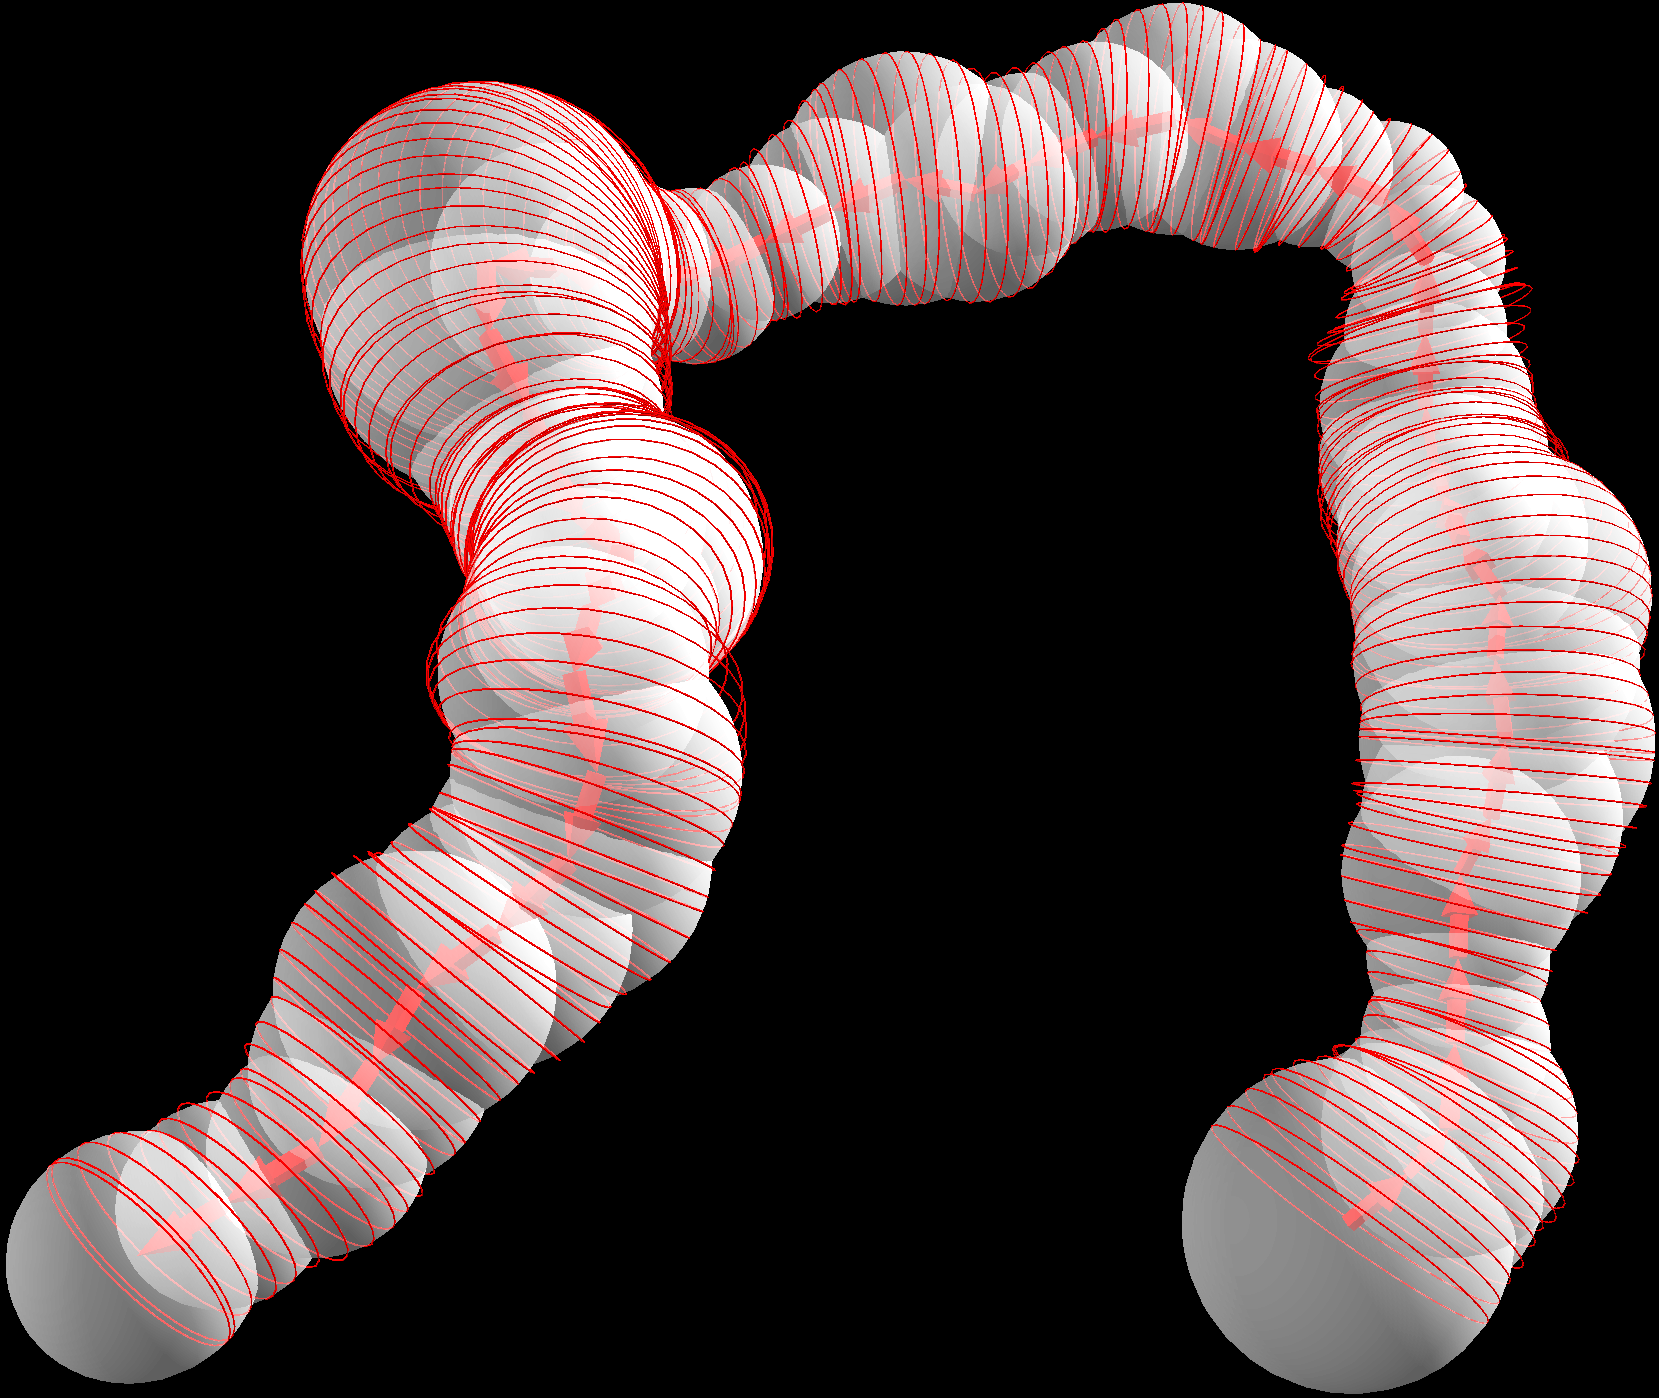
\includegraphics[width=1\textwidth]{img/1BRT.png}
    \caption{Diskretizace tunelu v enzymu Chloroperoxidase (1BRT).}
  \centering
  \label{fig:1BRT}
\end{figure}
